\section{Performance Analysis and Optimization in Privacy-Preserving Federated Learning}


\subsection{背景}

\subsubsection{挑战}

在FL中, 敌人可能会通过窃听和分析共享参数来攻击学习模型(重构攻击和推理攻击). 
例如, 恶意分类器可能揭示客户数据的特征, 并根据给定的FL模型重构数据点.  

超大数据量和隐私保护的要求下,联邦学习(FL)得到应用. 由于FL本地训练, 不要求客户上传他们的私人数据, 因此有效地减少了传输开销, 同时保护客户的隐私. 
因此, FL 适用于各种数据敏感或传输到服务器代价昂贵的情况, 例如, 医疗记录、私人图像和个人识别信息等. 
虽然 FL 可以保护私有数据不被公开, 但是 共享参数可能被窃取用来分析攻击模型(例如重构攻击和推理攻击). 

\paragraph{本文贡献}

利用本地差分隐私(Local DP), 引入客户端级别差分隐私(CDP)算法 

证明CDP在一定隐私水平下满足DP的要求,求出了CDP的理论收敛界.
 

\subsection{相关工作}
\begin{itemize} 
    \item Privacy-Preserving Deep Learning  \cite{shokri2015privacy}表明集中搜索数据仓库和开放数据应用的出现可能会导致私人信息的泄露. 
    % \item Deep Learning with Differential Privacy \cite{abadi2016DLwithDP}首次提出了差分隐私深度学习(DP)的概念, 为隐私保障提供了评价标准
    \item Privacy-Preserving Collaborative Deep Learning With Unreliable Participants  \cite{zhao2020collaborative}设计了一种函数机制, 在训练过程中扰动神经网络的目标函数, 以达到一定的DP水平
    \item Concentrated Differentially Private Gradient Descent with Adaptive per-Iteration Privacy Budget \cite{Lee2018ConcentratedDP}  改进了基于DP的随机梯度下降(SGD)算法, 在每次训练迭代中仔细分配隐私预算. 
    \item Differentially Private Distributed Online Learning \cite{Li2018DiffOnline}  引入数据处理的概念, 提出了一种分布式在线学习算法, 以提高在给定隐私水平下的学习性能
    \item Differentially Private Federated Learning: A Client Level Perspective \cite{Geyer2017Client} 提出了一个保护隐私的FL框架, 当有足够多的客户参与时, 可以在低性能损失的情况下保持一个给定的隐私水平. 
    \item A Hybrid Approach to Privacy-Preserving Federated Learning\cite{Truex:2019:HAP:3338501.3357370} 将DP与安全多方计算相结合 
    \item Privacy for Free: Communication-Efficient Learning with Differential Privacy Using Sketches \cite{li2019privacy}  提出基于sketches草图的FL框架, 为客户获得可证明的DP好处, 它可以将通过草图传输的消息压缩到很高的通信效率. 
    
草图算法(sketch)在数据集上提供不同统计数据(如计算不同的计数或平均值)的近似估计,并被广泛应用于流数据处理、数据库和网络测量。
草图也被用于大规模机器学习,如压缩模型更新,识别梯度向量中的重要坐标,减少模型训练中的内存使用。

最近, 的一些尝试考虑通过使用随机噪声、随机采样或其他随机方法来扩展草图,以提供差分隐私。
但是,他们需要在草图之上添加这些机制,并且不研究草图本身的任何固有的隐私属性。
分析表明,草图具有固有的不同的隐私属性,可以用于设计私有分布式学习算法,与最先进的机制相比,该算法能够实现更好的通信和准确性权衡
     
\end{itemize}

    以上工作提出了差分隐私, 给出隐私性能评价标准, 给出了设置一定隐私水平的目标函数的方法, 并利用分布式在线学习, 安全多方计算, Sketches 等方法概念, 提高联邦学习的计算性能隐私性能和通信效率. 

  
Calibrating Noise to Sensitivity in Private Data Analysis\cite{Dwork2006} 提出了根据敏感度来添加噪声实现差分隐私的方法. 证明可以通过根据函数f的灵敏度来校准噪声的标准偏差来保持隐私. 粗略地说, f的任何一个参数可以改变其输出的量. 


    下表\ref{tab:FLnotation}表示了本文常用的符号.
    \begin{figure}[!ht]
        \centering
        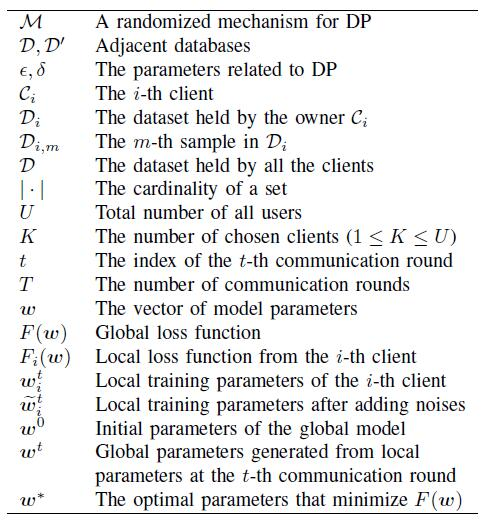
\includegraphics[width=0.6\textwidth]{CDP/notation.jpg}
        \caption{主要符号}
        \label{tab:FLnotation}
    \end{figure}
\subsection{预备知识}

 

\subsubsection{本地差分隐私}

传统的差分隐私是将原始数据集中到一个数据中心, 然后在此对数据施加差分隐私算法, 并对外发布, 称之为中心化差分隐私(Centralized Differential Privacy). 因此, 中心化差分隐私有一个前提: \textbf{可信的第三方数据收集者}, 即保证所收集的数据不会被窃取和泄露. 然而, 在实际生活中想找到一个真正可信的第三方数据收集平台十分困难, 这极大地限制了中心化差分隐私的应用. 

未解决以上问题本地化差分隐私,  基于不可信第三方的前提下, 其将数据隐私化的工作转移到每个用户, 用户自己来处理和保护个人数据, 极大地降低了隐私泄露的可能性. 
任意本地化差分隐私函数f, 定义域为$Dom(f)$, 值域为$Ran(f)$, 对任意输入$t, t^{'} \in Dom(f)$, 输出$t^{*} \in Ran(f)$, 都有:

$P[ f(t) = t^{*} ] \leq e^{\varepsilon }\times P[ f(t^{'}) = t^{*} ] $

本地化差分隐私技术通过控制任意两条记录的输出结果的相似性, 从而确保算法f满足本地化差分隐私, 即输出同为$t^{*}$, 窃密者无法确认输入为$t$还是$t^{'}$;
$\varepsilon$越小, 任意两条记录输出结果相似性越高. 

\begin{figure}[!ht]
    \caption{本地差分隐私}
    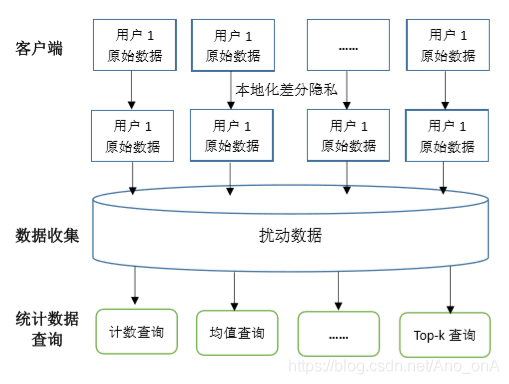
\includegraphics[width=0.8\textwidth]{CDP/LDP.png}
\end{figure}

\paragraph{Client Level Differentially Privacy }
(集中式)联邦学习情况下,受信任的管理者会聚合由多个客户以分散方式优化的参数。然后,产生的模型被分发回所有的客户端,最终在不显式共享数据的情况下汇聚成一个联合的代表模型。但是,该协议很容易受到不同攻击,这些攻击可能来自在联邦优化期间参与的任何一方。在这样的攻击中,通过分析分布式模型,客户在训练中的贡献和他们数据集的信息被揭示出来。针对这一问题,\cite{Geyer2017Client}提出了一种客户端差分隐私保护联邦优化算法。其目的是在训练期间隐藏客户的贡献,平衡隐私损失和模型性能之间的权衡。实证研究表明,如果\textbf{有足够多的参与客户,其提出的程序可以在模型性能上以很小的成本保持客户级别的差分隐私。}

\paragraph{该文的主要贡献:}在联邦学习中保持较高的模型性能时,可以隐藏客户的参与, 在轻微损失模型的性能下实现客户端级别差分隐私。
其次,提出在分布式训练中动态适应dp保护机制。 与集中式学习相比,联邦学习中的梯度在整个训练过程中对噪音和批量大小表现出不同的灵敏度。
\cite{McMahan2018Learning}提出了一个类似的客户级dp程序。不同的是其实验设置\cite{McMahan2018Learning}还包括元素级隐私措施。
\textbf{元素级隐私}

\paragraph{方法}
\begin{enumerate}
    \item \textbf{Random sub-sampling随机子抽样}
    \item \textbf{Distorting:} A Gaussian mechanism is used to distort the sum of all updates. This requires knowledge about the set’s sensitivity with respect to the summing operation. We can enforce a certain sensitivity by using scaled versions instead of the true updates:$w^t_i=max(1, \|  \frac{w^t_i}{S}\|)$. Scaling ensures that the second norm is limited $\forall k, \|w^t_i\|_2<S$. The sensitivity of the scaled updates with respect to the summing operation is thus upper bounded by S. The GM now adds noise (scaled to sensitivity S) to the sum of all scaled updates. Dividing the GM’s output by mt yields an approximation to the true average of all client’s updates, while preventing leakage of crucial information about an individual.

   缩放后的更新相对于求和运算的灵敏度因此上限为S。高斯机制将噪声(缩放到灵敏度S)加到所有缩放后的更新的和上。 
\end{enumerate}

\leader{R\'enyi Divergence}
\begin{definition}[{R\'enyi Divergence ]{ }}]
    Let $P$ and $Q$ be probability distributions on $\Omega$. For $\alpha \in  (1,\infty)$, we define the \emph{R\'enyi divergence of order $\alpha$ between $P$ and $Q$} as 
    \begin{align*}
    D_\alpha (P||Q)
     =& \frac{1}{\alpha - 1} \log \left( \int_\Omega P(x)^\alpha Q(x)^{1-\alpha} \mathrm{d} x \right) \\
     =& \frac{1}{\alpha-1} \log \left( \ex{x \sim Q}{ \left(\frac{P(x)}{Q(x)}\right)^\alpha} \right) \\
     =& \frac{1}{\alpha-1} \log \left( \ex{x \sim P}{ \left(\frac{P(x)}{Q(x)}\right)^{\alpha-1}} \right),
    \end{align*}


其中$P(\cdot)$ and $Q(\cdot)$ 分别是$P$和$Q$的概率质量/密度函数. 更一般地, $P(\cdot)/Q(\cdot)$ 是  $P$对于$Q$的Radon-Nikodym导数.\footnote{If $P$ is not absolutely continuous with respect to $Q$ (i.e. it is not the case that $P \ll Q$), we define $D_{\alpha}({P}||{Q})=\infty$ for all $\alpha \in [1,\infty]$.}

 
我们定义 KL-divergence $$\dr{1}{P}{Q} = \lim_{\alpha \to 1} \dr{\alpha}{P}{Q} = \int_\Omega P(x) \log \left(\frac{P(x)}{Q(x)}\right) \mathrm{d}x$$ 和 max-divergence $$\dr{\infty}{P}{Q} = \lim_{\alpha \to \infty} \dr{\alpha}{P}{Q} = \sup_{x \in \Omega} \log \left(\frac{P(x)}{Q(x)}\right) .$$

 R\'enyi divergence 可以被定义为$P$ 和 $Q$隐私损失  : $$e^{(\alpha-1)\dr{\alpha}{P}{Q}} = \ex{Z\sim\privloss{P}{Q}}{e^{(\alpha-1)Z}}$$ for all $\alpha \in (1,\infty)$. 而且, $\dr{1}{P}{Q} = \ex{Z\sim\privloss{P}{Q}}{Z}$.

    \end{definition}


\leader{计算S值} 

在每个通信轮中,计算所有未剪切梯度贡献的平均值,并使用它作为剪切界$S=median{\triangle w^k}_{k \in \mathbf{Z}_t}$. 

\subsubsection{威胁模型--需应对的问题}
\textbf{推理攻击}通过模型推断私有特征和\textbf{重构攻击}通过模型重构训练数据
在重构攻击中, 攻击者的目标是推断训练集中记录的属性. 
推理攻击中, 攻击者的目标是推断特定的个人数据记录是否包含在训练数据集中. 
\paragraph{本文假设}服务器诚实但好奇.即敌手诚实地遵守协议, 但也会试图从接受到的信息中学习除输出意外的信息. 

如下图\ref{fig:threatModel}所示,一个有诚实但好奇的服务器或窃听者的FL训练模型, 他们可以通过分析来自客户端的训练参数来推断私有特征并重建原始数据. 

\begin{figure}[!ht]
    \centering
    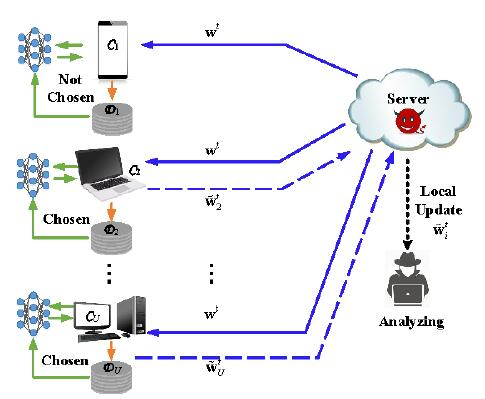
\includegraphics[width=0.5\textwidth]{CDP/threat.jpg}
    \caption{threat model}
    \label{fig:threatModel}
\end{figure}

\subsection{隐私和收敛性分析}


\subsubsection{Client-level DP 客户端级别DP}

\begin{figure}[!ht]
    \centering
    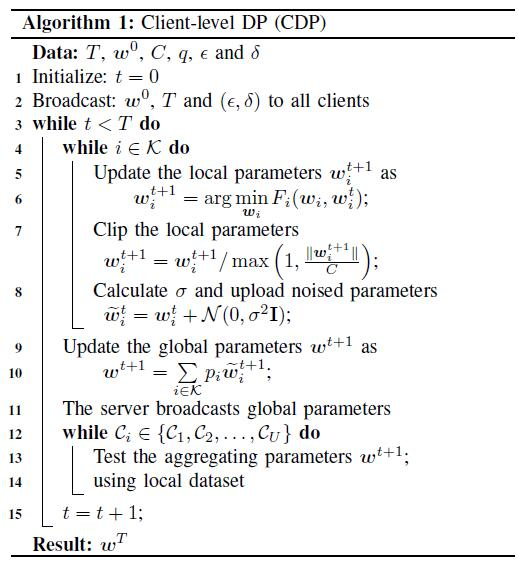
\includegraphics[width=0.6\textwidth]{CDP/alg_CDP.jpg}
    \caption{客户端级DP算法CDP}
    \label{fig:alg_CDP}
\end{figure}
其中,$T$表示通信轮数, $w^0$为初始化全局参数, $\sigma$为加性噪音的标准方差, q为随机抽样比率$K=| \mathcal{K}= qU|$. 

初始: 服务器向客户机初始化全局参数$w^0$

第t轮聚合: K个客户端完成$w$的局部训练, 利用阈值C进行裁剪, 向$w_i^{t+1}$增加噪音得到参数$\tilde{w}_i^{t+1}$并上传. $\tilde{w}_i^t=w_i^t + \mathcal{N}(0, \sigma^2I)$. 
之后,服务器更新全局参数$w^{t+1}$, 并广播. 客户端利用局部数据测试准确率并开始下一轮循环.
直至通讯轮数达到$T$.

\subsubsection{Bound of the Moment}
根据~\cite{abadi2016DLwithDP}, 使用高斯机制, 我们可以定义隐私损失
\begin{equation}
c \triangleq \exp\left(\alpha^{T}(\lambda)\right) = \exp\left(\sum_{t=1}^{T}\alpha(\lambda)\right),
\end{equation}
和矩生成函数
\begin{equation}
\alpha(\lambda) \triangleq \ln(\max \{D_{\nu_{1},\nu_{0}}, D_{\nu_{0},\nu_{1}}\}),
\end{equation}
其中$\lambda$ 是任意正整数, $\nu_{0}$ 为 $\mathcal{N}(0,\sigma^{2})$的概率密度函数(PDF), $\nu_{1}$ 表示 两个高斯分布 $q\mathcal{N}(\Delta s,\sigma^{2})+(1-q)\mathcal{N}(0,\sigma^{2})$的复合, $q=K/U$ 是随机取样率,
\begin{equation}
D_{\nu_{1},\nu_{0}}=\mathbb{E}_{z\sim \nu_{1}}\left(\frac{\nu_{1}}{\nu_{0}}\right)^{\lambda}=\mathbb{E}_{z\sim \nu_{0}}\left(\frac{\nu_{1}}{\nu_{0}}\right)^{\lambda+1},
\end{equation}
and
\begin{equation}
D_{\nu_{0},\nu_{1}}=\mathbb{E}_{z\sim \nu_{0}}\left(\frac{\nu_{0}}{\nu_{1}}\right)^{\lambda}=\mathbb{E}_{z\sim \nu_{0}}\left(\frac{\nu_{1}}{\nu_{0}}\right)^{-\lambda}.
\end{equation}

%We will use moments accountant method to keep track of a bound on the moments with random sampling. This method can provide a much tighter estimation of the privacy loss.

然而, ~\cite{abadi2016DLwithDP}中关于矩界的推导只能应用于严格约束$q \leq \frac{1}{16\sigma}$. 
为了解决这个问题, 我们提出~\textbf{Lemma~\ref{lemma:Comp_div}}来进一步约束该矩. 
\begin{lemma}

考虑到moments accountant法中使用的两种高斯分布$\nu_{0}$和$\nu_{1}$, 它们满足以下关系: 
\begin{equation}
D_{\nu_{1},\nu_{0}}\geq D_{\nu_{0},\nu_{1}}.
\end{equation}
\end{lemma}


\begin{figure}
    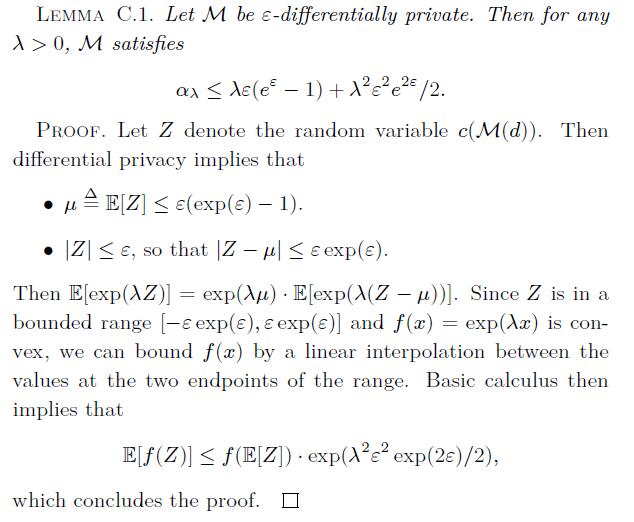
\includegraphics[width=0.9\textwidth]{figures/CDP/moment_bound.jpg}
\end{figure}

Privacy accounting:对于不同隐私的SGD来说, 一个重要的问题是计算训练的总体隐私成本. 不同隐私的可组合性使我们能够实现一个“accountant”程序, 计算每次访问训练数据时的隐私损失, 并累积这些成本. 
\cite{abadi2016DLwithDP, mcsherry2009privacy}
 
\subsubsection{敏感度和隐私分析}

相邻数据集:我们在第i个用户中考虑两个相邻的数据库$D_i, D_i^\prime \in\mathcal{X} $, 其中$Di$和$D0i$大小相同, 只相差一个样本. 
实值函数的敏感度可以表示为由于添加或删除单个样本,  函数值可能发生变化的最大程度. 
 
在本文中, 我们选择了采用$L_2$范数灵敏度的高斯机制, 函数$s$的灵敏度可以表示为
\begin{equation}
\Delta s = \max\Vert s(\mathcal D)-s(\mathcal D')\Vert_{2}.
\end{equation}
 
\paragraph{局部敏感度} 对于一个查询函数f , 它的形式为: $f : D \to \mathbb{R}$ , 其中D为一数据集, R 是查询函数的返回结果。在一给定的数据集D 和与它相邻的任意数据集$D'$上, 它的局部敏感度定义如下:

$LS_f=\max_{D'} \|f(D)-f(D')\|$

与全局敏感度不同, 局部敏感度是由查询函数和给定的数据集共同决定, 因为局部敏感度只是对于一个数据集做变化。因为局部敏感度限制了一对相邻数据集中的一个数据集, 所以如果在局部敏感度中, 给定的数据集和全局敏感度中使$\|f(D)-f(D')\|$达到最大的数据集相同时, 局部敏感度等于全局敏感度. 


\begin{assumption}
    假设局部训练中的批量大小等于训练样本的数量. 
    \label{assump1}
\end{assumption}


基于\ref{assump1},用梯度下降法,
\begin{figure}[!ht]
    \centering
    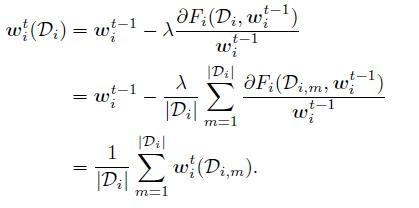
\includegraphics[width=0.6\textwidth]{CDP/generalGD.jpg}
\end{figure}
得到敏感度
$ \triangle l = \frac{2C}{D_i}$, 其中C是阈值.


\begin{theorem}
    给定采样比q和通信轮数T,保证$(\varepsilon, \delta)-DP$对于训练数据集中使用的所有数据, 高斯机制噪声扰动的STD应该满足
$$\sigma= \frac{\sqrt{2qT\ln(1/\delta)} }{\varepsilon}$$
\end{theorem}

 将等式21换为20, 有$\sigma^{t+1}= \sigma^t$.

 CRD算法可以总结为以下
\begin{assumption}
    \begin{figure}[!ht]
        \centering
        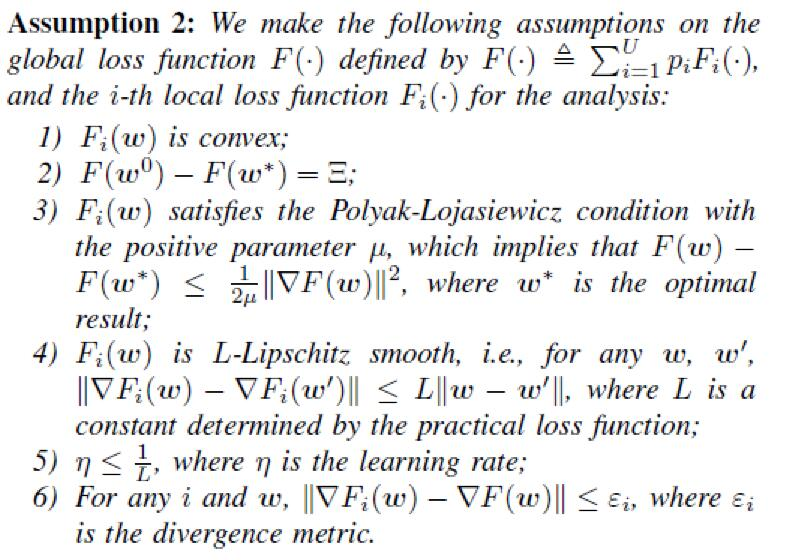
\includegraphics[width=0.7\textwidth]{CDP/assump2.jpg}
    \end{figure}
\end{assumption}

\begin{theorem}
    \label{theorem2}
    \begin{figure}[!ht]
        \centering
        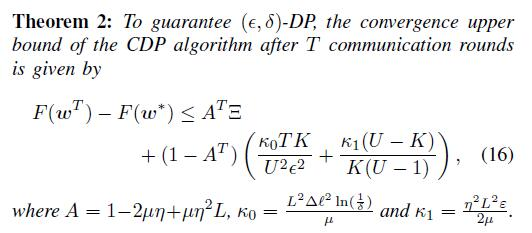
\includegraphics[width=0.8\textwidth]{CDP/theorem2.jpg}
    \end{figure}
\end{theorem}
理论\ref{theorem2} 显示了收敛性能和隐私之间的精确权衡:当隐私保证较弱时,收敛边界较小, 表明收敛到最优权值的收敛. 从我们的假设中, 我们知道$\eta L  \leqslant 1, \ A <1 $.


\subsection{CDP中的折扣DISCOUNTING方法}

当训练性能停止提高时,稍微降低T的值,可以得到更小的STD,从而提高性能. 
据此,作者提出CRD算法(communication rounds discounting). 在CRD中, T是迭代确定的. 如图\ref{fig:alg_CDP}所示,表现了带CRD的CDP算法在第t轮通信的训练过程.

步骤1, 初始化: 服务器广播$w^0$初始参数,$T, \upsilon \text{和}\delta$;

步骤2, 局部训练

步骤3, 梯度剪裁: 为了证明DP保证,每个例子对当地的影响参数应与限幅阈值有界c.每个参数向量将在L2范数范围内. 如第i个局部参数向量$w^t_i$在第t轮沟通被$w^t_i=max(1, \|  \frac{w^t_i}{C}\|)$替换(这种参数剪裁形式在SGD和ML常用.
由于差分隐私保护要求限制每个样本对最终梯度$\tilde{g}_t$的影响。鉴于梯度的取值范围无先验
限定,故采用$L_2$范数首先对每个梯度进行裁剪, 
裁剪后结果为:若$\|g\|_2 \leq C$,则保留g,若$\|g \|_2 > C$,则将其缩小为常量C。进行隐私损失累积操作的主要目的在于跟踪计算每次训练迭代过程中的隐私损失成本。可以根据所加噪声的分布参数进而确定每次叠加过程的隐私损失$α(\delta)$。

步骤4, 添加噪声: 具有确定STD的人工高斯噪声将被添加到本地训练参数保证$(\upsilon,\delta)-\text{DP}$; 本地参加噪声区别于中心化差分隐私.
步骤5, 参数上传

步骤6, 模型聚合

步骤7, 模型广播: 服务器广播聚合的参数和通信轮数T给所有客户端;

步骤8,模型更新:所有客户更新各自与聚合模型参数,然后测试的性能更新模型和性能上传到服务器;

步骤9:通信轮折扣:当停止提高收敛性能, 服务器的折现方法将被触发. 服务器将获得一个小于前一个T的线性折扣因子. 这个因素可以控制T的衰减速度, 当聚合时间达到预设的T时, 联邦学习过程结束. 

  

梯度范数剪切阈值的选取需要综合考虑如下两个因素:1) 若阈值取值过小,则最终以平均值代替真实梯度时可能造成误差过大;2) 若阈值取值过大,则由算法1 可知,将会导致最终根性的梯度中注入过多的噪声。
\begin{figure}[!ht]
    \centering
    \FloatBarrier
    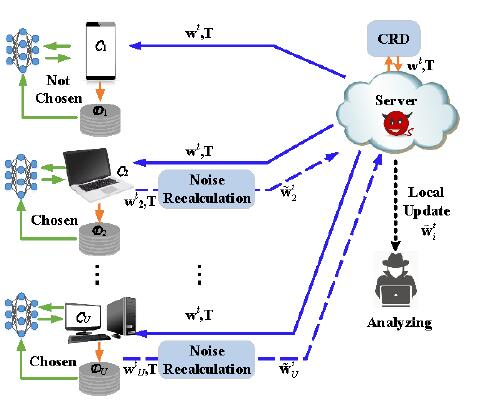
\includegraphics[width=0.8\textwidth]{CDP/CRD.jpg}
    \caption{使用CRD方法训练CDP第t轮通信中过程}
    \label{CRD}

\end{figure}
 

\subsubsection{T的噪声重计}

\begin{theorem}
    \label{theorem3}
    \begin{figure}[ht]
        \centering
        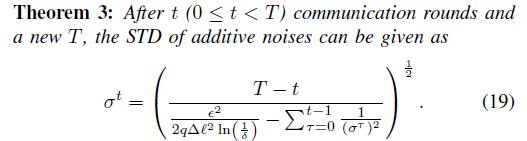
\includegraphics[width=0.8\textwidth]{CDP/theorem3.jpg}
    \end{figure}
\end{theorem}

基于前面的训练过程和T的值, 我们可以获得一个有合适的STD的噪声. ($\sigma^\tau$小)
如果在前面的训练过程有较大STD(强隐私保证), 重新计算后的STD将小(弱隐私保证).($\sigma^t$小)
如果在这轮通信中T的值不变, 那么STD的值将保持不变. 
考虑$\sigma^t, \sigma^{t+1}$和不变的T,从上面的方程,可得
\begin{figure}[!ht]
    \centering
    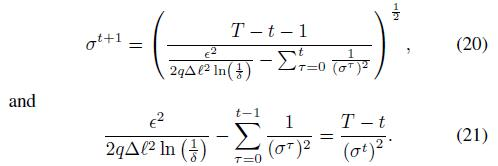
\includegraphics[width=0.6\textwidth]{CDP/equation2021RecalT.jpg}
\end{figure} 

\begin{figure}[ht]
    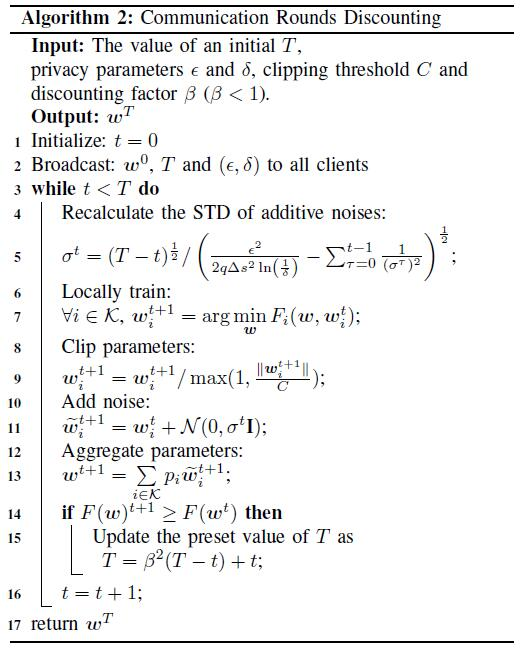
\includegraphics[width=0.7\textwidth]{CDP/alg_code_CRD.jpg}
    \label{alg_code_CRD}
    \caption{CDP with CRD method}
\end{figure}
    在\ref{alg_code_CRD}中,有CRD方法的详细步骤.

\subsection{实验}
\subsubsection{结果评价}

\begin{figure}[ht]
    \centering
    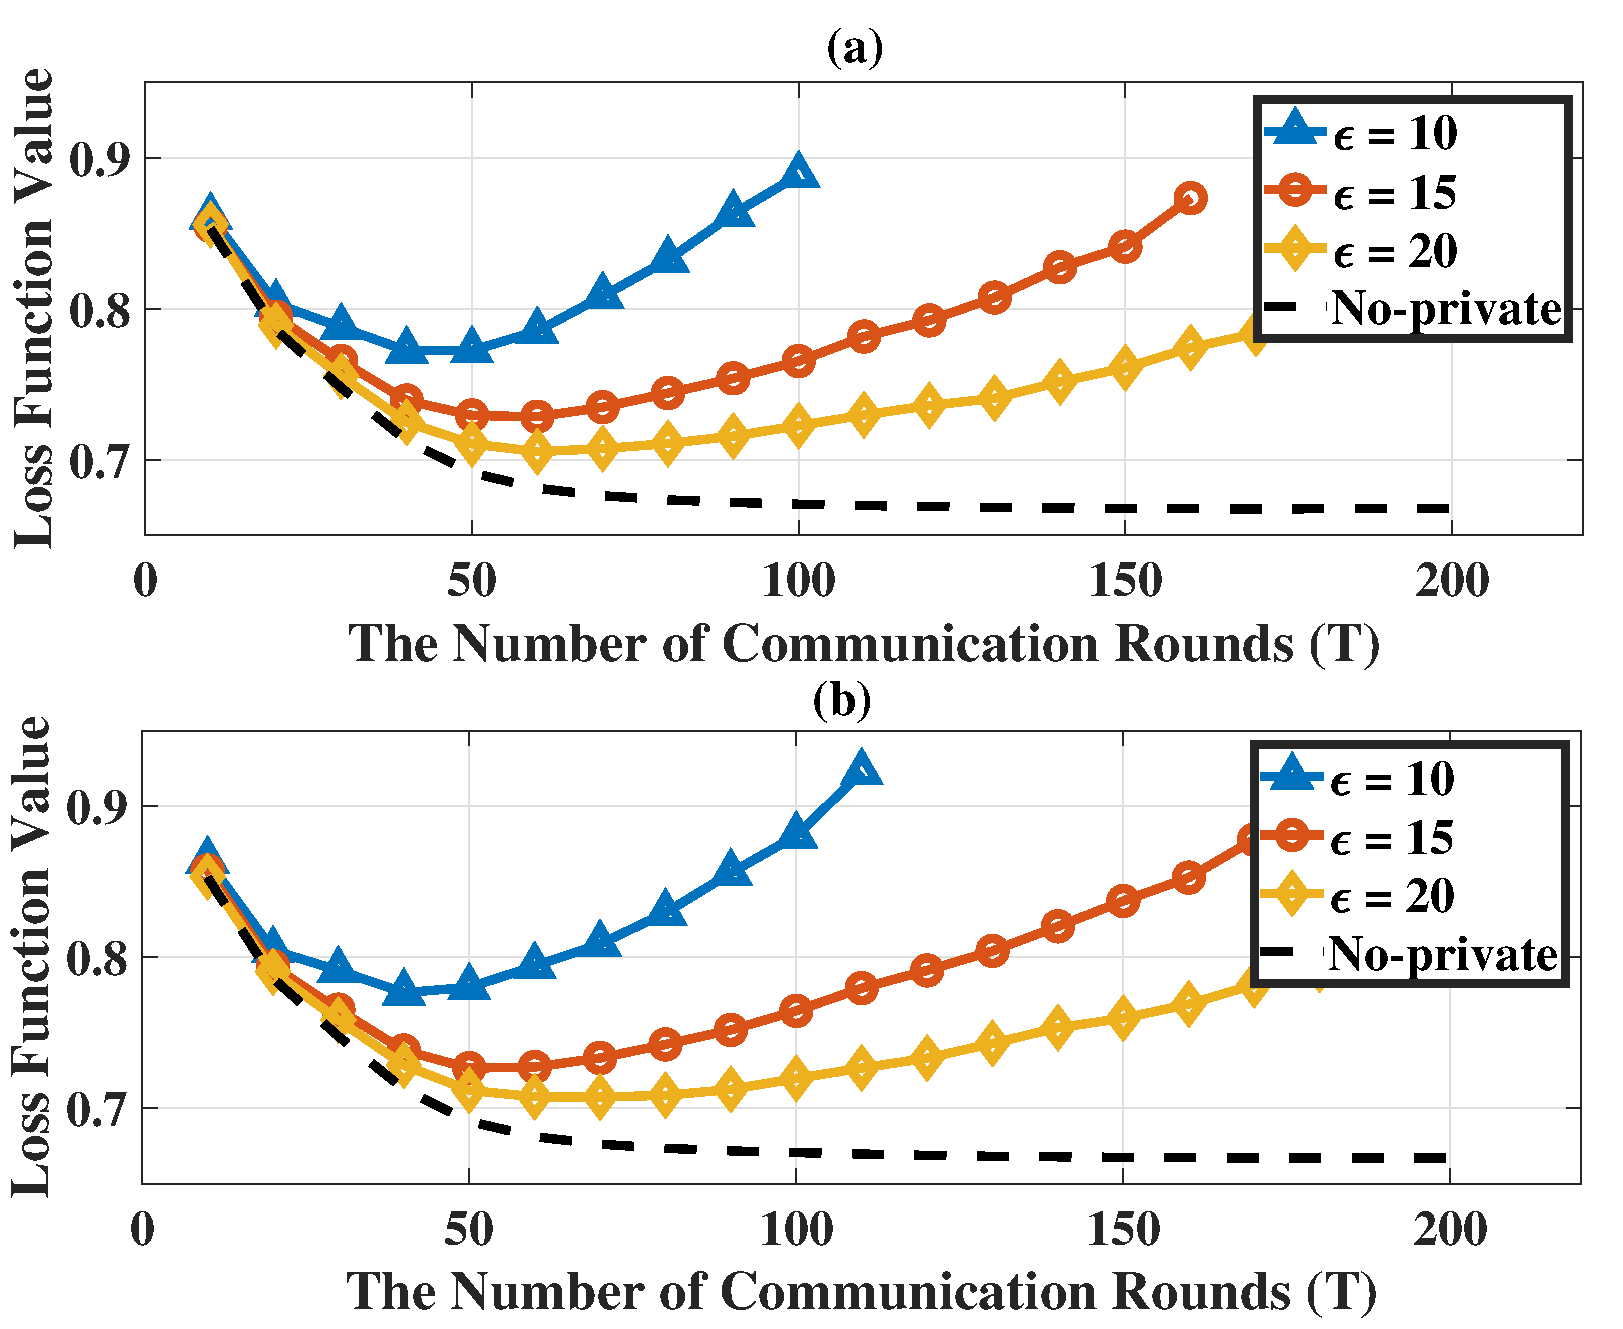
\includegraphics[width=3.2in,angle=0]{figures/CDP/Svm_ConvforNandK_T.pdf}
    \caption{Value of the loss function under various $T$ using the CDP algorithm (SVM). (a) $U=50, K=50$ ($q=1$). (b) $U=50, K=30$ ($q=0.6$).}
    \label{fig:SVM_ConvforNandK_T}
    \end{figure}

    \begin{figure}[ht]
    \centering
    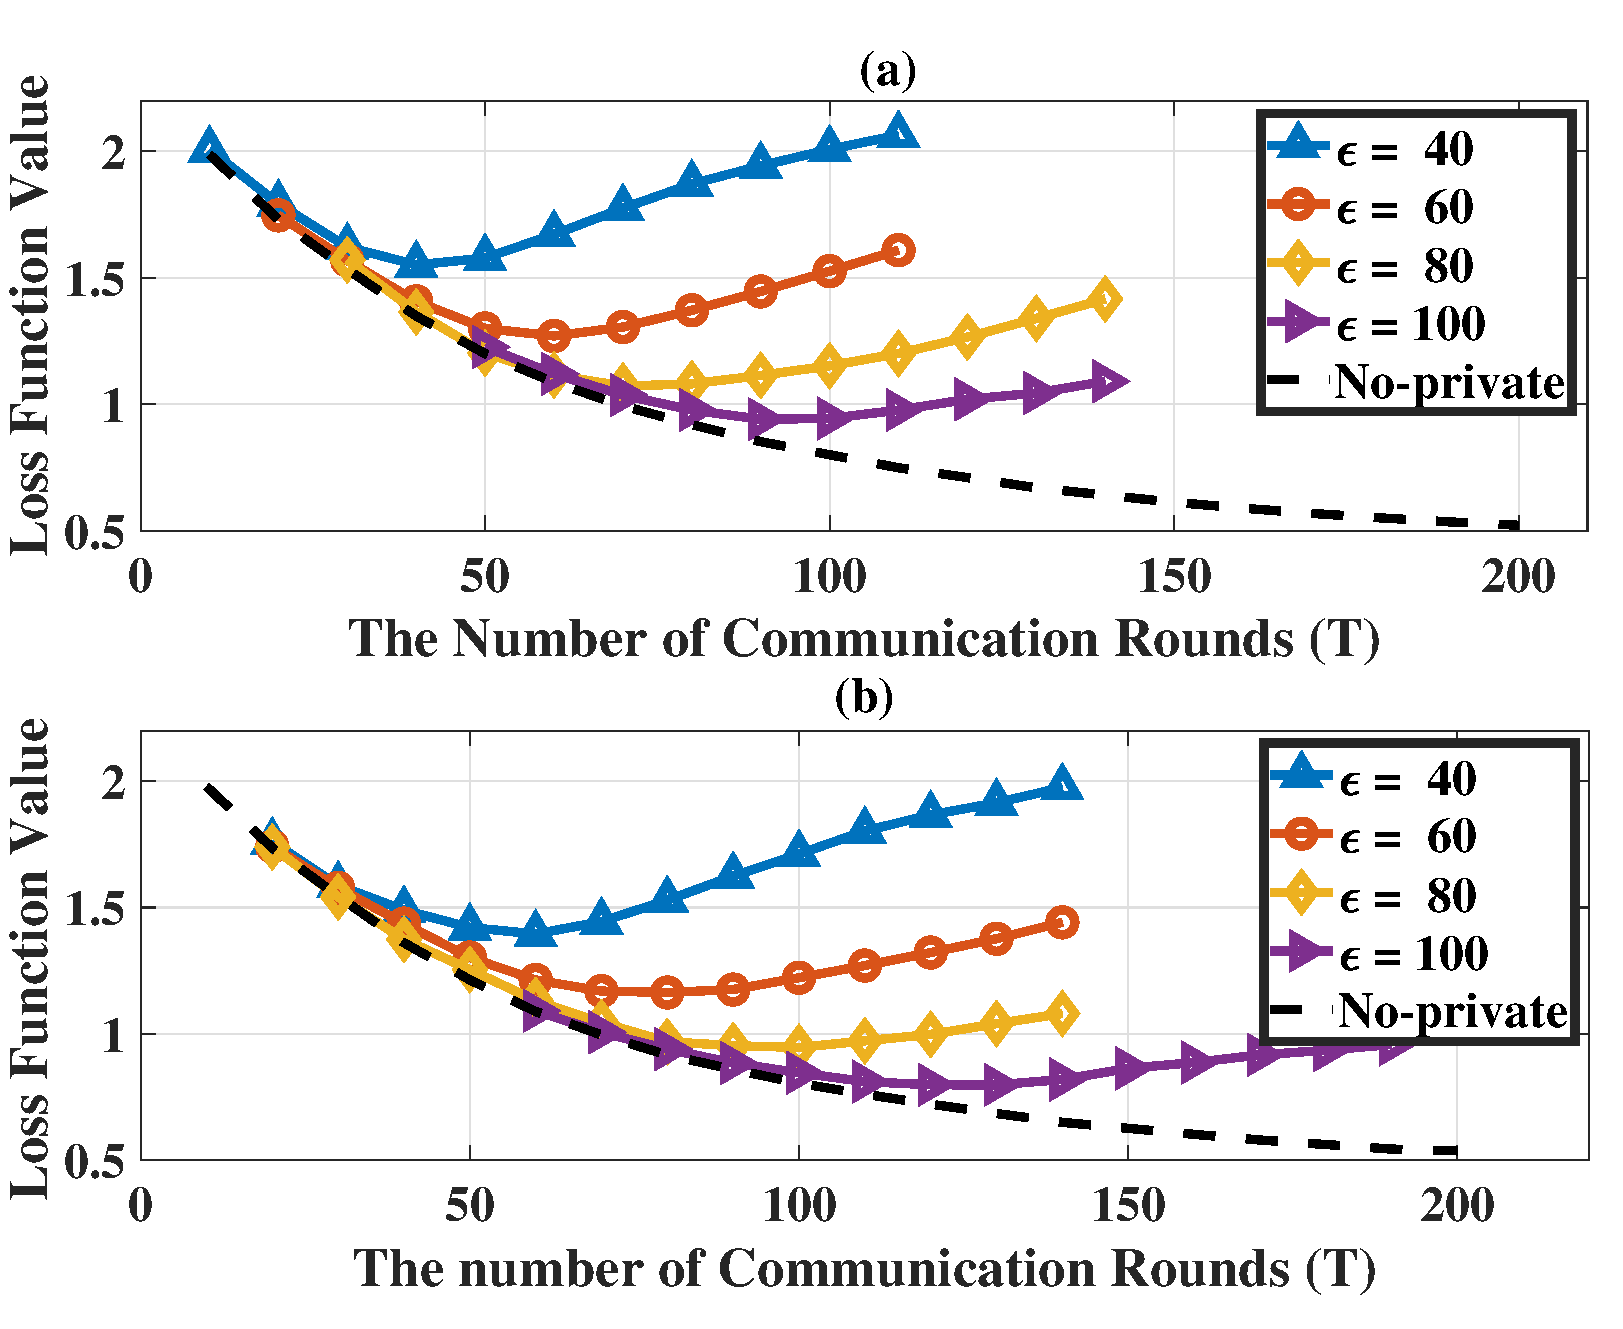
\includegraphics[width=3.2in,angle=0]{figures/CDP/ConvforKandN_T.pdf}
    \caption{Value of the loss function under various $T$ using the CDP algorithm (MLP). (a) $U=50, K=50$ ($q=1$). (b) $U=50, K=30$ ($q=0.6$).}
    \label{fig:MLP_ConvforNandK_T}
    \end{figure}

    \begin{figure}[ht]
    \centering
    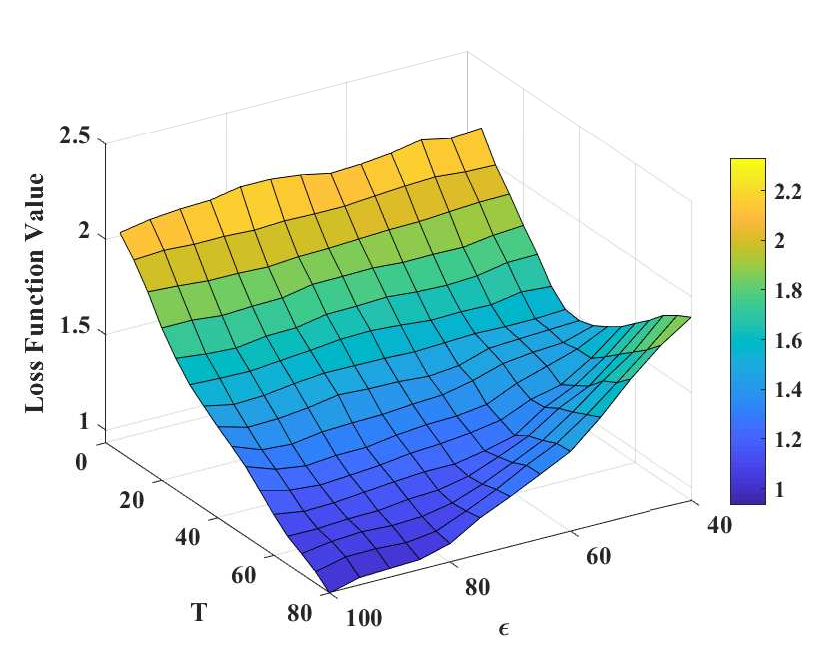
\includegraphics[width=3.2in,angle=0]{figures/CDP/ConvforN_T_eps_td.pdf}
    \caption{Value of the loss function under various $T$ and privacy levels using the CDP algorithm (MLP) with $U=K=50$ ($q=1$).}
    \label{fig:ConvforN_T_eps_td}
    \end{figure}

    \begin{figure}[ht]
    \centering
    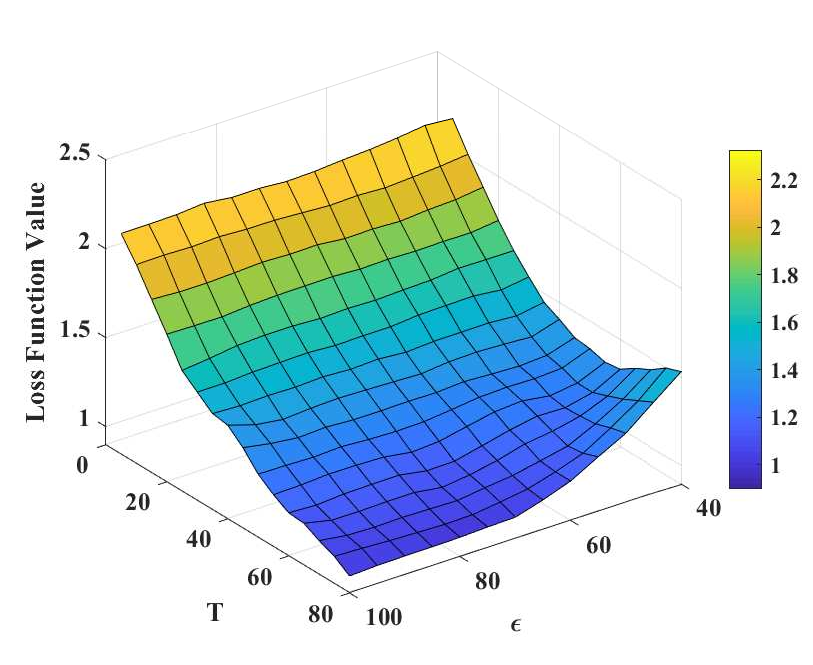
\includegraphics[width=3.2in,angle=0]{figures/CDP/ConvforK_T_eps_td.pdf}
    \caption{Value of the loss function under various $T$ and privacy levels using the CDP algorithm (MLP) with $U=50$ and $K=30$ ($q=0.6$).}
    \label{fig:ConvforK_T_eps_td}
    \end{figure}
    Fig~\ref{fig:ConvforN_T_eps_td}和~\ref{fig:ConvforK_T_eps_td} 用来说明抽样的作用.

Fig~\ref{fig:ConvforN_T_eps_td}和~\ref{fig:ConvforK_T_eps_td}通过改变隐私级别$\epsilon$和$T$的值, 说明了使用MLP模型在FL中的CDP算法训练损失函数值的期望. 从图~\ref{fig:ConvforN_T_eps_td}可以看出, 没有采样, 较大的$T$和较小的$\epsilon$性能糟糕. 如图~\ref{fig:ConvforN_T_eps_td}中采样比$q=0.6$的第二种情形所示, 它也可以保持同样的性质. 

抽样和批量随机梯度下降法类似.
作者用SVM和MLP模型来验证理论结果.  观察结果与Remark 1 一致, 其因为较低的隐私水平降低了附加噪声的标准差, 服务器可以从客户端获得更好质量的ML模型参数. 从 \ref{fig:SVM_ConvforNandK_T} 和图\ref{fig:MLP_ConvforNandK_T} 中,可以看出T的最优值几乎随着$\varepsilon$的增加而增加. 

 
\subsubsection{对CRD的评价}
\paragraph{T初始化}
当T更接近T的最优值时, 会得到更好的收敛性能.
\paragraph{隐私级别}
更小的隐私水平使用CRD方法更早结束. T越大, 信息泄漏的可能性越大, 附加噪声的STD越大. 之后, CRD方法可能被触发, 减小的T将从服务器广播到客户端. 
\paragraph{折扣因子} 当隐私级别固定时, 较大的$\beta$会导致T较慢的衰减速度,意味着在训练中仔细调整T有利于收敛性能. 更仔细的调整将导致更多的通信回合消耗. 最优CDP具有最好的收敛性能, 但需要消耗大量的通信轮数. 最终结论:通过选择多路切换, 在通信周期消耗和收敛性能之间存在一个折衷.  
\textbf{未来待研究:解析地评估损失函数最小的最优值. }

\subsection{结论}
本文为解决联邦学习训练中防止共享参数被窃取导致隐私泄露的情况, 设计CDP算法保护隐私, 并进一步通过折扣法提高训练效率, 且从理论上得出该算法的上界. 最后根据实验评价通信轮数T, 隐私水平参数 $\varepsilon$, 折扣因子$\beta$对算法的影响. 
算法重点如下:
引入本地差分隐私, 根据灵敏度得到剪切阈值,并据此设计满足$(\varepsilon,\delta)-DP$的加噪高斯机制. 

提出CRD折扣法, 收敛性能稳定时触发该机制, 并自动优化参数T, 并动态更改加噪方差, 进一步获得更优模型. 









 
 


\subsection{公式推导}

\subsubsection{Bound of the Moment 矩界}

\begin{algorithm}[htb]
	\caption{Differentially private SGD (Outline)}\label{alg:privsgd}
	\begin{algorithmic}
	\REQUIRE Examples $\{x_1,\ldots,x_N\}$,\\ loss function $\calL(\btheta)=\frac{1}{N}\sum_i \calL(\btheta, x_i)$. \\ Parameters: learning rate $\eta_t$, noise scale $\sigma$, group size $L$, gradient norm bound $C$. 
%\bmnote{Give a formula for choosing $\sigma_t$. Also: why two Input: (\REQUIRE) lines?}
%LZ: we are adopting the strategy of choosing sigma and then using privacy
%accountant to accumulate the privacy loss. Maybe we should make that more
%explicit in Privacy Accountant section?
		\STATE {\bf Initialize} $\btheta_0$ randomly
		\FOR{$t \in [T]$}
		\STATE {Take a random sample $L_t$ with sampling probability $L/N$}
		\STATE {\bf Compute gradient}
		\STATE {For each $i\in L_t$, compute $\bfg_t(x_i) \gets \nabla_{\btheta_t} \calL(\btheta_t, x_i)$}		
		\STATE {\bf Clip gradient}
		\STATE {$\bar{\bfg}_t(x_i) \gets \bfg_t(x_i) / \max\big(1, \frac{\|\bfg_t(x_i)\|_2}{C}\big)$}
		\STATE {\bf Add noise}
		\STATE {$\tilde{\bfg}_t \gets \frac{1}{L}\left( \sum_i \bar{\bfg}_t(x_i) + \mathcal{N}(0, \sigma^2 C^2 \Id)\right)$}
		\STATE {\bf Descent}
		\STATE { $\btheta_{t+1} \gets \btheta_{t} - \eta_t \tilde{\bfg}_t$}
		\ENDFOR
		\STATE {\bf Output} $\btheta_T$ and compute the overall privacy cost $(\eps, \delta)$ using a privacy accounting method.
%\bmnote{Ref to Eqs or pseudocode for computing privacy cost.}
%LZ: we will spend most of time discussing how privacy is computed. Since
%the algorithm description is an outline, maybe we can postpone it?
	\end{algorithmic}
\end{algorithm}

\begin{theorem}
      \label{thm:momentBound}
	存在常数 $c_1$ and $c_2$ 使 已知抽样概率  $q=L/N$以及步数$T$, 对于任意$\eps < c_1 q^2T$, 如果我们选择以下$\sigma$值, 算法~\ref{alg:privsgd} 对于任意$\delta>0$  是 $(\eps,\delta)$-DP,  
	\begin{align*}
	\sigma \geq c_2\frac{q \sqrt{T \log(1/\delta)}}{\eps}\,.
	\end{align*}
\end{theorem}

根据~\cite{abadi2016DLwithDP}, 使用高斯机制, 我们可以定义隐私损失
\begin{equation}
c \triangleq \exp\left(\alpha^{T}(\lambda)\right) = \exp\left(\sum_{t=1}^{T}\alpha(\lambda)\right),
\end{equation}
和矩生成函数
\begin{equation}
\alpha(\lambda) \triangleq \ln(\max \{D_{\nu_{1},\nu_{0}}, D_{\nu_{0},\nu_{1}}\}),
\end{equation}
其中$\lambda$ 是任意正整数, $\nu_{0}$ 为 $\mathcal{N}(0,\sigma^{2})$的概率密度函数(PDF), $\nu_{1}$ 表示 两个高斯分布 $q\mathcal{N}(\Delta s,\sigma^{2})+(1-q)\mathcal{N}(0,\sigma^{2})$的复合, $q=K/U$ 是随机取样率,
\begin{equation}
D_{\nu_{1},\nu_{0}}=\mathbb{E}_{z\sim \nu_{1}}\left(\frac{\nu_{1}}{\nu_{0}}\right)^{\lambda}=\mathbb{E}_{z\sim \nu_{0}}\left(\frac{\nu_{1}}{\nu_{0}}\right)^{\lambda+1},
\end{equation}
和
\begin{equation}
D_{\nu_{0},\nu_{1}}=\mathbb{E}_{z\sim \nu_{0}}\left(\frac{\nu_{0}}{\nu_{1}}\right)^{\lambda}=\mathbb{E}_{z\sim \nu_{0}}\left(\frac{\nu_{1}}{\nu_{0}}\right)^{-\lambda}.
\end{equation}

%We will use moments accountant method to keep track of a bound on the moments with random sampling. This method can provide a much tighter estimation of the privacy loss.

然而, ~\cite{abadi2016DLwithDP}中关于矩界的推导只能应用于严格约束$q \leq \frac{1}{16\sigma}$. 
为了解决这个问题, 我们提出~\textbf{Lemma~\ref{lemma:Comp_div}}来进一步约束该矩. 
\begin{lemma}\label{lemma:Comp_div}

考虑到矩会计法中使用的两种高斯分布$\nu_{0}$和$\nu_{1}$, 它们满足以下关系: 
\begin{equation}
D_{\nu_{1},\nu_{0}}\geq D_{\nu_{0},\nu_{1}}.
\end{equation}
\end{lemma}

 
Privacy accounting:对于不同隐私的SGD来说, 一个重要的问题是计算训练的总体隐私成本. 不同隐私的可组合性使我们能够实现一个“accountant”程序, 计算每次访问训练数据时的隐私损失, 并累积这些成本. 



\subsection{理论1的证明}
 
差分隐私保证转为moment bound矩界.

\newtheorem{thm_appendix}{Theorem}[section]
\newtheorem{lem_appendix}[thm_appendix]{Lemma}
\begin{lem_appendix}
  \label{lem:pure_dp_to_logmgf}
  Let $\calM$ be $\eps$-differentially private. Then for any $\lambda > 0$, $\calM$ satisfies
\begin{align*}
\alpha_{\lambda} \leq \lambda\eps(e^{\eps}-1) + \lambda^2\eps^2e^{2\eps}/2.
\end{align*}
  \end{lem_appendix}
\begin{proof}
  Let $Z$ denote the random variable $c(\calM(d))$. Then differential privacy implies that
  \begin{itemize}
      \item $\mu \eqdef \E[Z] \leq \eps(\exp(\eps) - 1)$.  
      \item $|Z| \leq \eps$, so that $|Z-\mu| \leq \eps \exp(\eps)$.
    \end{itemize}
  Then $\E[\exp(\lambda Z)] = \exp(\lambda\mu) \cdot \E[\exp (\lambda(Z-\mu))]$. Since $Z$ is in a bounded range $[-\eps\exp(\eps), \eps\exp(\eps)]$ and $f(x) = \exp(\lambda x)$ is convex, we can bound $f(x)$ by a linear interpolation between the values at the two endpoints of the range. Basic calculus then implies that
  \begin{align*}
    \E[f(Z)] \leq f(\E[Z]) \cdot \exp(\lambda^2 \eps^2 \exp(2\eps)/2),
    \end{align*}
 which concludes the proof.
 \end{proof}
\mycomment{Similarly,
\begin{lemma}
  \label{lem:approx_dp_to_logmgf}
  Let $\calM$ be $(\eps,\delta)$-DP. Then $\calM$ is $(\lambda\eps(e^{\eps}-1) + \lambda^2\eps^2e^{2\eps}/2, \delta, \lambda)$-logmgf bounded.
  \end{lemma}
}
 
\setcounter{theorem}{1}\begin{theorem}\label{thm:property_supp}
    Let $\alpha_\calM(\lambda)$ defined as \[\alpha_\calM(\lambda) \eqdef \max_{\aux, d, d'} \alpha_\calM(\lambda; \aux, d, d'),\]
    最大值被接收所有的辅助输入和邻近的数据库$d,d'$,那么有
    
    \begin{enumerate}
    \item \textbf{[Composability]}
    Suppose that a mechanism $\calM$ consists of a sequence of adaptive mechanisms $\calM_1, \ldots, \calM_k$ where $\calM_i\colon \prod_{j=1}^{i-1}\Range_j\times \Domain \to\Range_i$. Then, for any $\lambda$
    \[\alpha_\calM(\lambda) \leq \sum_{i=1}^k \alpha_{\calM_i}(\lambda)\,.\]
    
    \item \textbf{[Tail bound]}
    For any $\eps>0$, the mechanism $\calM$ is $(\eps, \delta)$-differentially private for
    \[\delta=\min_{\lambda} \exp(\alpha_\calM(\lambda) -\lambda \eps)\,.\]
    \end{enumerate}
    \end{theorem}
     

Lemma~\ref{lem:pure_dp_to_logmgf}和Theorem~\ref{thm:property_supp}给出了一种获得差分机制的组合定理的方法,这大致相当于展开~\cite{Dwork2010boosting}的强组合定理的证明。\logmgfa会计的有效性是因为,对于许多选择的机制,直接限制界在\logmgfa 比建立差异隐私和应用Lemma~\ref{lem:pure_dp_to_logmgf}有更强的保证。\cite{abadi2016DLwithDP, mcsherry2009privacy}

定义 $\mu_{0} \triangleq \mathcal{N}(0,\sigma)$, $\mu_{1} \triangleq \mathcal{N}(\Delta\ell,\sigma)$, $\nu_{0} \triangleq \mathcal{N}(0,\sigma)$ 且 $\nu_{0} \triangleq q\mu_{0}+(1-q)\mu_{1}$.

有 $\mathcal M(\mathcal{D})\sim \nu_0$ and $\mathcal M(\mathcal{D}')\sim \nu_1$.
第$\lambda$阶矩 $\alpha(\lambda_{n})$可表示为

\begin{equation}
\alpha(\lambda) = \ln\max \left\{D_{\nu_{0}, \nu_{1}}, D_{\nu_{1},\nu_{0}}\right\},
\end{equation}
其中
\begin{equation}
D_{\nu_{1},\nu_{0}}=\mathbb{E}_{z\sim \nu_{1}}\left(\frac{\nu_{1}}{\nu_{0}}\right)^{\lambda}\, \text{and}\,D_{\nu_{0},\nu_{1}}=\mathbb{E}_{z\sim \nu_{0}}\left(\frac{\nu_{0}}{\nu_{1}}\right)^{\lambda}.
\end{equation}
这里界定 $D_{\nu_{0}, \nu_{1}}$ 和 $D_{\nu_{1},\nu_{0}}$.

基于 ~\textbf{Lemma~\ref{lemma:Comp_div}},考虑 $D_{\nu_{1},\nu_{0}}$, 有
\begin{equation}
\begin{aligned}
&D_{\nu_{1},\nu_{0}}=\mathbb{E}_{z\sim \nu_{1}}\left(\frac{\nu_{1}}{\nu_{0}}\right)^{\lambda}\\
&=\int_{-\infty}^{+\infty} \nu_0\left(1-q+qe^{\frac{2z\Delta s-\Delta \ell^{2}}{2\sigma^{2}}}\right)^{\lambda+1} \mathrm{d}z\\
&=\int_{-\infty}^{+\infty} \nu_0
\sum_{l=0}^{\lambda+1}\left(\begin{matrix}\lambda+1\\ l\end{matrix}\right)(1-q)^{\lambda+1-l}q^le^{\frac{l\left(2z\Delta\ell-\Delta \ell^{2}\right)}{2\sigma^{2}}}\mathrm{d}z\\
&=
\sum_{l=0}^{\lambda+1}\left(\begin{matrix}\lambda+1\\ l\end{matrix}\right)(1-q)^{\lambda+1-l}q^{l}e^{\frac{l(l-1)\Delta \ell^{2}}{2\sigma^{2}}}\\
&\leq\left(1-q+qe^{\frac{\lambda\Delta s^{2}}{2\sigma^{2}}}\right)^{\lambda+1}\leq e^{q(\lambda+1)\left(e^{\frac{\lambda\Delta \ell^{2}}{2\sigma^{2}}}-1\right)}.\\
\end{aligned}
\end{equation}
假设 $\frac{\lambda\Delta\ell^{2}}{2\sigma^{2}}\ll1$ for $\lambda \in [1,T]$, 有
\begin{equation}\label{equ:divergence_bound}
D_{\nu_{1},\nu_{0}} \leq e^{q(\lambda+1)\left(\frac{\lambda\Delta\ell^{2}}{2\sigma^{2}}+O\left(\frac{\lambda^{2}\Delta \ell^{4}}{4\sigma^{4}}\right)\right)}\approx e^{\frac{q\lambda(\lambda+1)\Delta\ell^{2}}{2\sigma^{2}}}.
\end{equation}
由以上的矩, 有
\begin{equation}\label{equ:moments}
\alpha^{T}(\lambda) \leq \sum_{t=1}^{T}\alpha(\lambda, \sigma)=\frac{Tq\lambda(\lambda+1)\Delta\ell^{2}}{2\sigma^{2}}.
\end{equation}
使用矩的下界\cite{abadi2016DLwithDP}, 有
\begin{equation} 
\delta = \min_{\lambda}\exp\left(\alpha^{T}(\lambda)-\lambda\epsilon\right)
=\min_{\lambda}\exp\left(\frac{Tq\lambda(\lambda+1)\Delta\ell^2}{2\sigma^2}-\lambda\epsilon\right).
\end{equation}

\begin{equation}
\frac{Tq\lambda(\lambda+1)\Delta\ell^2}{2\sigma^2}-\lambda\epsilon=\frac{Tq\Delta\ell^{2}}{2\sigma^2}\left(\lambda+\frac{1}{2}-\frac{\epsilon\sigma^2}{Tq\Delta\ell^2}\right)^2-\frac{Tq\Delta s^{2}}{2\sigma^2}\left(\frac{1}{2}-\frac{\epsilon\sigma^2}{Tq\Delta\ell^2}\right)^2.
\end{equation}
设$\lambda = \frac{\epsilon\sigma^2}{Tq\Delta\ell^2}-\frac{1}{2}$, 有
\begin{equation}
\delta \geq\exp\left(-\frac{Tq\Delta\ell^{2}}{2\sigma^2}\left(\frac{1}{2}-\frac{\epsilon\sigma^2}{T\Delta\ell^2}\right)^2\right).
\end{equation}
因此
\begin{equation}
\ln(\delta)\geq-\frac{Tq\Delta\ell^{2}}{2\sigma^2}\left(\frac{1}{2}-\frac{\epsilon\sigma^2}{Tq\Delta\ell^2}\right)^2,
\end{equation}
然后有
\begin{equation}
\ln\left(\frac{1}{\delta}\right)\leq\frac{Tq\Delta\ell^{2}}{2\sigma^2}\left(\frac{1}{2}-\frac{\epsilon\sigma^2}{Tq\Delta\ell^2}\right)^2
=\frac{Tq\Delta\ell^{2}}{8\sigma^2}-\frac{\epsilon}{2}+\frac{\epsilon^2 \sigma^2}{2Tq\Delta\ell^{2}}.
\end{equation}
由于$\delta \in (0,1)$,可知  
\begin{equation}\label{appendix:A_2}
\frac{Tq\lambda(\lambda+1)\Delta\ell^2}{2\sigma^2}-\lambda\epsilon<0.
\end{equation}
结合~\eqref{appendix:A_2}, 将 $\ln\left(1/\delta\right)$约束为
\begin{equation}
\ln\left(\frac{1}{\delta}\right)<-\frac{\epsilon}{4}+\frac{\epsilon^2 \sigma^2}{2Tq\Delta\ell^{2}}<\frac{\epsilon^2 \sigma^2}{2Tq\Delta \ell^{2}}.
\end{equation}
选择满足
\begin{equation}\label{Appendix_C_1}
\sigma = \frac{\Delta \ell\sqrt{2qT\ln\left(\frac{1}{\delta}\right)}}{\epsilon}.
\end{equation} 的 $\sigma$ 保证联邦学习架构中的 $(\epsilon, \delta)$-DP. 
定理1 量化了噪音等级和隐私等级的关系. 噪音越多($\sigma$越大), 隐私性能越高($\epsilon$越小),且可以看出, 通讯轮数越多, 需要添加的噪音就要更多 才能保证相同的隐私水平.

\textbf{公式18的证明}

\subsection{proof of Theorem 2} \label{appendix:ConvforK}
定义
\begin{equation}\label{equ:K_aggregation}
\mathbf{w}^{t+1} \triangleq \sum_{i \in \mathcal{K}}{p_{i}\widetilde{\mathbf{w}}_{i}^{t+1}}=\sum_{i \in \mathcal{K}}{p_{i}(\mathbf{w}_{i}^{t+1}}+\mathbf{n}^{t+1}_{i}),
\end{equation}
和
\begin{equation}
\mathbf{n}^{t+1} \triangleq \sum_{i \in \mathcal{K}}p_{i}\mathbf{n}^{t+1}_{i}.
\end{equation}
进行二阶泰勒展开
\begin{equation}\label{equ:taylor_expan}
F(\mathbf{w}^{t+1})-F(\mathbf{w}^{t})\leq (\mathbf{w}^{t+1}-\mathbf{w}^{t})^{\top}\nabla F(\mathbf{w}^{t})\\
+\frac{L}{2}\Vert \mathbf{w}^{t+1}-\mathbf{w}^{t}\Vert^{2}.
\end{equation}
因为
\begin{equation}\label{equ:gd}
\mathbf{w}_{i}^{t+1}=\mathbf{w}^{t}-\eta \nabla F_{i}(\mathbf{w}^{t}).
\end{equation}
替换不等式\eqref{equ:gd} and  \eqref{equ:K_aggregation}  为\eqref{equ:taylor_expan}, 则有~\eqref{equ:long_equ2}.
\begin{figure*}[ht]
\normalsize
\begin{equation}\label{equ:long_equ2}
\begin{aligned}
F(\mathbf{w}^{t+1})- F(\mathbf{w}^{t})&\leq \left(\mathbf{n}^{t+1}-\eta\sum_{i\in \mathcal{K}}{p_{i}\nabla F_{i}(\mathbf{w}^{t})}\right)^{\top}\nabla F(\mathbf{w}^{t})+\frac{L}{2}\Vert \sum_{i\in \mathcal{K}}{p_{i}(\mathbf{n}_{i}^{t+1}-\eta\nabla F_{i}(\mathbf{w}^{t}))}\Vert^{2}\\
&=\frac{\eta^2L}{2}\Vert \sum_{i\in \mathcal{K}}{p_{i}\nabla F_{i}(\mathbf{w}^{t})}\Vert^{2}-
\eta\nabla F(\mathbf{w}^{t})^{\top}\sum_{i\in \mathcal{K}}{p_{i}\nabla F_{i}(\mathbf{w}^{t})}
+\frac{L}{2}\Vert\sum_{i\in \mathcal{K}}p_{i}\mathbf{n}_{i}^{t+1}\Vert^2.
\end{aligned}
\end{equation}
\hrulefill
\end{figure*}
 $F(\mathbf{w}^{t+1})$  可表示为
\begin{multline}\label{equ:exp_obj}
\mathbb{E}\{F(\mathbf{w}^{t+1})\}\leq F(\mathbf{w}^{t})-\eta\Vert \nabla F(\mathbf{w}^{t})\Vert^{2}\\
+\frac{\eta^2L}{2}\mathbb{E}\{\Vert \sum_{i\in \mathcal{K}}{p_{i}\nabla F_{i}(\mathbf{w}^{t})}\Vert^{2}\}
+\frac{L}{2}\mathbb{E}\{\Vert\mathbf{n}^{t+1}\Vert^2\}.
\end{multline}

假设 $p_{i} = 1/K$,
\begin{equation}
\label{equ:ConvforK_0}
\begin{aligned}
 \mathbb{E}\{\Vert \sum_{i\in \mathcal{K}}{p_{i}\nabla F_{i}(\mathbf{w}^{t})}\Vert^{2}\} &= \frac{1}{UK}\sum_{i\in \mathcal{U}}{\Vert \nabla F_{i}(\mathbf{w}^{t})\Vert^{2}}
+\frac{K-1}{UK(U-1)}\sum_{i\in \mathcal{U}}\sum_{j\in \mathcal{U}/i}{\left[\nabla F_{i}(\mathbf{w}^{t})\right]^{\top}\nabla F_{j}(\mathbf{w}^{t})}\\
\ &=\left(\frac{1}{UK}-\frac{K-1}{UK(U-1)}\right)\sum_{i\in \mathcal{U}}{\Vert \nabla F_{i}(\mathbf{w}^{t})\Vert^{2}}
+\frac{K-1}{UK(U-1)}\left(\sum_{i\in \mathcal{U}}\nabla F_{i}(\mathbf{w}^{t})\right)^2\\
\ &= \frac{U-K}{UK(U-1)}\sum_{i\in \mathcal{U}}{\Vert \nabla F_{i}(\mathbf{w}^{t})\Vert^{2}}+\frac{U(K-1)}{K(U-1)}\Vert\nabla F(\mathbf{w}^{t})\Vert^2.
\end{aligned} 
\end{equation}
由假设2,
\begin{multline}
\mathbb{E}\{\varepsilon_{i}\}=\frac{1}{U}\sum_{i\in \mathcal{U}}\varepsilon_{i}=\frac{1}{U}\sum_{i\in \mathcal{U}}{\Vert \nabla F_{i}(\mathbf{w}^{t})-\nabla F(\mathbf{w}^{t})\Vert^{2}} \\
=\frac{1}{U}\sum_{i\in \mathcal{U}}{\Vert \nabla F_{i}(\mathbf{w}^{t})\Vert^{2}}-\Vert\nabla F(\mathbf{w}^{t})\Vert^2
\end{multline}
替换$\mathbb{E}\{\varepsilon_{i}\}$ 为~\eqref{equ:ConvforK_0},  有\eqref{equ:upper_bound}.
\begin{figure*}[htb]
\normalsize
\begin{multline}\label{equ:upper_bound}
\mathbb{E}\{\Vert \sum_{i\in \mathcal{K}}{p_{i}^{\mathcal{K}}\nabla F_{i}(\mathbf{w}^{t})}\Vert^{2}\}
=\frac{U-K}{UK(U-1)}\sum_{i\in \mathcal{N}}{\Vert \nabla F_{i}(\mathbf{w}^{t})-\nabla F(\mathbf{w}^{t})\Vert^{2}}
+\Vert\nabla F(\mathbf{w}^{t})\Vert^2
\leq\frac{(U-K)\varepsilon}{K(U-1)}+\Vert\nabla F(\mathbf{w}^{t})\Vert^2.
\end{multline}

\end{figure*}
替换不等式\eqref{equ:upper_bound}  为\eqref{equ:exp_obj}, 有

\begin{multline}
\label{Appendix_D_1}
\mathbb{E}\{F(\mathbf{w}^{t+1})\}\leq F(\mathbf{w}^{t})-\eta\left(\frac{\eta L}{2}-1\right)\Vert \nabla F(\mathbf{w}^{t})\Vert^{2}\\
+\frac{L}{2}\mathbb{E}\{\Vert\mathbf{n}^{t+1}\Vert^{2}\}+\frac{(U-K)\varepsilon}{K(U-1)} \\
\leq +\eta\left(\frac{\eta L}{2}-1\right)\Vert \nabla F(\mathbf{w}^{t})\Vert^{2}\\
+F(\mathbf{w}^{t})+\frac{L}{2}\mathbb{E}\{\Vert\mathbf{n}^{t+1}\Vert^{2}\}+\frac{\eta^{2} L(U-K)\varepsilon}{2K(U-1)}.
\end{multline}
替换$F(\mathbf{w}^{*})$ 为\eqref{Appendix_D_1}, 有~\eqref{Appendix_D_2}.
\begin{figure*}[htb]
\normalsize
\begin{equation}\label{Appendix_D_2}
\begin{aligned}
\mathbb{E}\{F(\mathbf{w}^{t+1})\}-F(\mathbf{w}^{*})\leq \mathbb{E}\{F(\mathbf{w}^{t})\}-F(\mathbf{w}^{*})+\frac{\eta^{2} L(U-K)\varepsilon}{2K(U-1)}+\eta\left(\frac{\eta L}{2}-1\right)\Vert \nabla F(\mathbf{w}^{t})\Vert^{2}+\frac{L}{2}\mathbb{E}\{\Vert\mathbf{n}^{t+1}\Vert^{2}\}.
\end{aligned}
\end{equation}
%\hrulefill
\vspace*{4pt}
\end{figure*}
递归应用 Polyak-Lojasiewicz 条件和 \eqref{Appendix_D_2}, a然后考虑添加噪音的独立性, 有
\begin{equation}
F(\mathbf{w}^{t})-F(\mathbf{w}^{*})\leq \left(1-2\mu\eta+\mu\eta^{2}L\right)^{t}(F(\mathbf{w}^{0})-F(\mathbf{w}^{*}))\\
+\frac{L^2(1-(1-2\mu\eta+\mu\eta^{2}L)^{t})}{2\mu}\bigg{(}\mathbb{E}\{\Vert\mathbf{n}\Vert^{2}\}\\
+\frac{\eta^{2} (U-K)\varepsilon}{K(U-1)}\bigg{)}.
\end{equation}

替换不等式\eqref{Appendix_C_1} 为上述不等式, 有
\begin{equation}
    \begin{aligned}
F(\mathbf{w}^{t})-F(\mathbf{w}^{*})\leq & \left(1-2\mu\eta+\mu\eta^{2}L\right)^{t}(F(\mathbf{w}^{0})-F(\mathbf{w}^{*}))\\
& +\frac{L(1-(1-2\mu\eta+\mu\eta^{2}L)^{t})}{\mu}\left(\frac{L\Delta\ell^{2}qt\ln(1/\delta)}{U\epsilon^{2}}\right. \\
& \left.+\frac{\eta^{2} L(U-K)\varepsilon}{2K(U-1)}\right).
\end{aligned}
\end{equation}
最终有收敛边界
\begin{equation}
F(\mathbf{w}^{t})-F(\mathbf{w}^{*})\leq A^{t}\Xi
+(1-A^t)\left(\frac{\kappa_{0}tK}{U^2\epsilon^2}+\frac{\kappa_{1}U(U-K)}{K(U-1)}\right),
\end{equation}
其中 $A = 1-2\mu\eta+\mu\eta^{2}L$, $\kappa_{0} = \frac{L^2\Delta\ell^2\ln(\frac{1}{\delta})}{\mu}$, $\kappa_{1} = \frac{\eta^{2} L^{2}\varepsilon}{2\mu}$. 
  
